% This must be in the first 5 lines to tell arXiv to use pdfLaTeX, which is strongly recommended.
\pdfoutput=1
% In particular, the hyperref package requires pdfLaTeX in order to break URLs across lines.

\documentclass[11pt]{article}

% Remove the "review" option to generate the final version.
% \usepackage[review]{emnlp2021}
\usepackage{emnlp2021}

% Standard package includes
\usepackage{times}
\usepackage{latexsym}

% For proper rendering and hyphenation of words containing Latin characters (including in bib files)
\usepackage[T1]{fontenc}

% This assumes your files are encoded as UTF8
\usepackage[utf8]{inputenc}
\usepackage{microtype}

% ======================================================================
% PEC For some reason the EMNLP templates put LH column line numbers on
% the right side. This switches them to the left side.
\usepackage[switch]{lineno} % default option is 'left
% ======================================================================

% PEC additions
\usepackage{graphicx}

\newcommand{\eat}[1]{}
\newcommand{\red}[1]{\textcolor{red}{#1}}
\newcommand{\blue}[1]{\textcolor{blue}{#1}}
\newcommand{\orange}[1]{\textcolor{orange}{#1}}
\newcommand{\green}[1]{\textcolor{ForestGreen}{#1}}
\newcommand{\teal}[1]{\textcolor{teal}{#1}}
\newcommand{\magenta}[1]{\textcolor{magenta}{#1}}
\usepackage{quoting}
\newenvironment{myquote}{                   % list without par spacings
  \parskip 0mm \begin{quoting}[vskip=0mm,leftmargin=2mm]}{
\end{quoting}}
\newenvironment{ite}{                     % list without par spacings
     \parskip 0cm \begin{itemize} \parskip 0cm \parsep 0cm \itemsep 0cm \topsep 0cm}{
        \end{itemize}} %  \parskip 0cm}
\newenvironment{enu}{                   % list without par spacings
     \parskip 0cm \begin{list}{}{\parsep 0cm \itemsep 0cm \topsep 0cm}}{
       \end{list}} %  \parskip 0cm}
\newenvironment{des}{                 % list without par spacings
     \parskip 0cm \begin{list}{}{\parsep 0cm \itemsep 0cm \topsep 0cm}}{
       \end{list}} %  \parskip 0cm}
\newenvironment{myenumerate}{                   % list without par spacings
     \parskip 0cm \begin{enumerate}{\parsep 0cm \itemsep 0cm \topsep 0cm}}{
        \end{enumerate}} %  \parskip 0cm}
\newenvironment{myitemize}{                     % list without par spacings
     \parskip 0cm \begin{itemize}{\parsep 0cm \itemsep 0cm \topsep 0cm}}{
        \end{itemize}} %  \parskip 0cm}

% ======================================================================

% If the title and author information does not fit in the area allocated, uncomment the following
%
%\setlength\titlebox{<dim>}
%
% and set <dim> to something 5cm or larger.

\title{Endowing Language Models with a Notion of Belief (?)}

% Author information can be set in various styles:
% For several authors from the same institution:
% \author{Author 1 \and ... \and Author n \\
%         Address line \\ ... \\ Address line}
% if the names do not fit well on one line use
%         Author 1 \\ {\bf Author 2} \\ ... \\ {\bf Author n} \\
% For authors from different institutions:
% \author{Author 1 \\ Address line \\  ... \\ Address line
%         \And  ... \And
%         Author n \\ Address line \\ ... \\ Address line}
% To start a seperate ``row'' of authors use \AND, as in
% \author{Author 1 \\ Address line \\  ... \\ Address line
%         \AND
%         Author 2 \\ Address line \\ ... \\ Address line \And
%         Author 3 \\ Address line \\ ... \\ Address line}

\author{Nora Kassner, Hinrich Sch{\"u}tze \\
Center for Information and Language Processing \\
LMU Munich, Germany \\
\texttt{kassner@cis.lmu.de} \\ \And
Oyvind Tafjord, Peter Clark \\
Allen Institute for AI \\
Seattle, WA \\
\texttt{\{oyvindt,peterc\}@allenai.org} \\
}

\begin{document}
\maketitle
\begin{abstract}
Although language models (LMs) have become adept at question-answering (QA), they
still can produce inconsistent answers, 
% Below - need to acknowledge there's already work on consistency reduction
even after using specialized training techniques to reduce model inconsistency. As a result, it can be hard to identify
% making it hard to identify  - old version
what the model actually
"believes" about the world. Our goal is to reduce this problem, so LMs are 
more globally consistent in their answers. Our approach is to add a memory
component - a BeliefBank - that records a model's raw answers and improves
consistency among them by flipping answers that significantly clash with others.
We show that, in a controlled experimental setting where facts are simple
propositions (e.g., "eagles are birds"), both accuracy and consistency
is improved. We also show that, by recalling pertinent beliefs from the
BeliefBank as context for new questions, raw answer accuracy for those unseen
questions is also improved. This feeds more accurate answers back into the growing
BeliefBank, creating a dynamic cycle of interaction between the model and BeliefBank.
This is significant as it is a first step towards endowing models with an evolving,
persistent memory, and creating systems that continuously improve over time.
\end{abstract}


\red{Why experiments are slow:
\begin{itemize}
    \item calibration is a problem!!! When I extended the dataset the calibration seems to not work well. I changed it to a heurisitc alternative which seems to work but that mean I have to rerun all SAT solving experiments
    \item SAT solving takes per entity: 
    \item each run of the full graph takes > 1h
    \item + 10 plants: 10 h
    \item + 20 incremental with random context: 20
    \item + 20 incremental with bm25 context: 20
\end{itemize}}

\red{What are the current issues:
\begin{itemize}
    \item If calibration is of F1 can still improve but it flips essential things from no-->yes and random things from yes-->no
    \item What kind of F1 should I report? Derivable facts (small test set but large improvements), gold facts (even smaller test set with good model performance and only small improvements, all IsA facts (might include a couple of wrong labels, large test set, only slight improvements as many nodes need more mututal exclusive connectivity)
    \item I have to filter plurals
    \item BM25 vs random retrieval: random seems to be better than BM25???
\end{itemize}}

\section{Introduction}

% \vspace{-1mm}
\begin{figure}[t]
\centering
     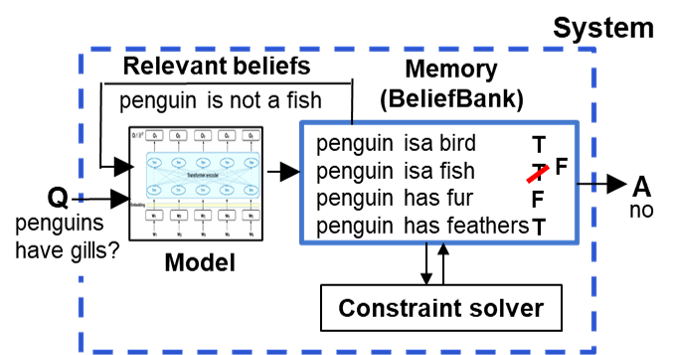
\includegraphics[width=1\columnwidth]{architecture2.png}	   % small figure
%      \vspace{-3mm}
\caption{The proposed architecture. The model's raw answers are stored in a
persistent memory (BeliefBank), and potentially flipped if they clash
significantly with others. Pertinent beliefs are then used to help the model answer new
questions. We find the consistency and accuracy of both the model and the overall
system improves with time. \label{architecture}}
% \caption{The proposed architecture. A memory layer (the BeliefBank)
% plus constraint solver improves the consistency of beliefs.
% Given a new question, relevant beliefs are recalled to help improve
% the model's answers, thus feeding more accurate results back into the BeliefBank.
% \label{arcuitecture}}
% \vspace{-3mm}
\end{figure}

How might we ascribe a notion of belief to a model? Prior work has shown that, while
models have high question-answering (QA) accuracy, they can also be inconsistent in their
answers, making it hard to pin down what a model actually ``believes'' about a proposition.
Our goal is to reduce this problem by having systems provide more globally consistent
answers to questions.

Prior work on reducing inconsistency has focused on retraining the model itself to be
more consistent, e.g., \cite{Ribeiro2019AreRR,Li2019ALF}, but with imperfect results. We present an
alternative approach in which the model is unchanged, but an evolving, persistent memory
of beliefs - called the BeliefBank - is layered on top, and can be used
to reduce inconsistency of the overall system (model + BeliefBank). Further,
we show how beliefs from the BeliefBank can be used as additional model
input for new questions, resulting in improved model answer accuracy,
and hence more accurate new beliefs for the BeliefBank. This allows the
overall system (model + BeliefBank) to continuously improve performance over
time, without retraining the model itself.

We explore this in a controlled experimental setting where 
both candidate facts and candidate constraints are provided. Candidate facts are simple
sentences that may be true or false, e.g., "An eagle is a bird" (T), ``An eagle is a mammal'' (F). Candidate constraints are between (variabilized) facts, e.g., ``?X is a bird $\rightarrow$ ?X can fly''. These allow us both to probe and measure improvement
in the system's consistency and accuracy, described shortly.

\red{Delete/reword this paragraph} Our approach involves an interplay between a model's raw answers, and an
evolving memory - the BeliefBank - of beliefs based on the model's earlier answers
and a set of constraints that should hold. Model's answers contribute to the BeliefBank,
and the BeliefBank contribute new context to help with future question-answering by
the model. In between, a constraint system serves to identify and reduce inconsistency
among beliefs in the BeliefBank. Combined, this results in a system capable of
continuous improvement over time, opening new possibilities for dialog and
interactive teaching.

\red{List contributions}

\section{Related work}

While there has been some prior work on improving answer consistency, the primary approach
has been through modified model training. \citet{Ribeiro2019AreRR} improved consistency
by adding question paraphrases and question implications to the training data (data augmentation).
Others have trained models with (small) {\it sets} of examples with known constraints
between them, and included an additional loss term reflecting inconsistency among
set members during training \cite{Minervini2018AdversariallyRN,Li2019ALF,Asai2020LogicGuidedDA}.
However, the constraints are unused at test time (beyond what the model may have
internalized), and inconsistent answers are still produced.

For problems requiring a structured answer, e.g., predicting a sequence of
state changes, domain-specific constraints have been used to downgrade/block
answers that violate them \cite{Tandon2018ReasoningAA,Du2019BeCI}. This
encourages consistency within a single answer structure, but not among
different answers, our goal here.

Concerning improving global consistency using constraints,
in the area of knowledge graph construction
% , where individual extractions may be noisy, 
\citet{Pujara2013KnowledgeGI} define ``knowledge graph identification''
as the task of building a maximally consistent knowledge graph given noisy facts
and their extraction confidences, and ontological constraints between them.
They develop a solution use probabilistic soft logic (PSL) \cite{Broecheler2010ProbabilisticSL}
as their constraint reasoner. 
Similarly \citet{berant2010global} learn the globally
optimal set of entailments between a large database of candidate
entailment pairs (with associated confidences), by applying
a global transitivity constraint (X$\vdash$Y \& Y$\vdash$Z $\rightarrow$ X$\vdash$Z)
with Integer Logic Programming. Our constraint solver performs an analogous
function in our architecture, using the Z3 SAT solver (Section~\ref{??}).

While there are neural architectures that include an associated dynamic memory,
e.g., \cite{Henaff2017TrackingTW,Sukhbaatar2015EndToEndMN}, these components
typically play the role of a short-term working memory to help computation.
In contrast, our BeliefBank memory layer is a persistent, long-term memory of
explicit beliefs.

% \red{Possibly cite \cite{Graves2016HybridCU} - the memory there is more like
% an opaque expansion of the original network. I'm inclined not to cite this though
% as it's old and not really relevant.}

% \subsection{PLMs and knowledge}
\subsection{Faithfulness}
\citet{subramanian-etal-2020-obtaining}
introduce the concept of module-wise faithfulness, a systematic evaluation of faithfulness in neural module networks for reasoning. We show that naive training does not produce faithful modules and propose several techniques to improve module-wise faithfulness. 

\eat{Work on \textbf{consistency in other domains}
includes \citep{du2019consistent} where  prediction
consistency in procedural text is improved. \citet{ribeiro-etal-2020-beyond} use consistency for more robust evaluation. \citet{li-etal-2019-logic} measure and mitigate inconsistency in natural language inference (NLI), and finally, \citet{camburu2020make} propose a method for measuring inconsistencies in NLI explanations \cite{camburu2018snli}.}

\eat{
\subsection{PLMs and KGs}
\subsection{Knowledge Graph Identification}
\citet{Pujara2013KnowledgeGI}
use probabilistic soft logic (PSL) \cite{Broecheler2010ProbabilisticSL}.
}

\subsection{Inconsistencies in KGs}
(copied from old paper, need rewrite)
Consistency in KBs has been
studied in theoretical frameworks in the context of the
satisfiability problem and KB construction, and efficient
algorithms for detecting inconsistencies in KBs have been
proposed \cite{hansen2000probabilistic,andersen2001easy}.
Other work aims to quantify the degree to which KBs are
inconsistent and detects inconsistent statements
\cite{Thimm:2009d,muino2011measuring,Thimm:2013}.
\cite{zhang2020need} showed that capturing factual knowledge inside PLMs is a specially resource hungry task.





\section{Problem Definition}

\subsection{Beliefs}

What does it mean to believe a proposition, say p = eagles are birds? In general, a system can
be said to (appear to) believe something if it acts as if it were true. In the specific
context of a QA system, we would expect it to produce answers consistent with p (and
its other beliefs). Pragmatically, we expect the system to (a) give a consistent answer to
different paraphrases of the question "p?" ("Are eagles birds?", "Is an eagle a type of bird?", ...),
and (b) give correct answers about implications of p ("Eagles lay eggs", "Eagles have feathers", ...),
conditional on the system knowing such implications and how to apply them.
% For example,
% if a system believes eagles are birds, and knows birds lay eggs (plus the rule of inheritance),
% we would expect it to answer "yes" to a question about whether eagles lay eggs.
Of course, a system may not perfectly answer such implications as the implications
may have exceptions, or the system may not be a perfect reasoner.\footnote{Similarly,
people do not always behave fully consistently with their professed beliefs.}.
Thus, to the external observer, there are {\it degrees} to which a system acts as if it
believes something.
% (Note this is distinct from a system's internal confidence in a belief).

% As has been shown elsewhere, language models (LM) can be inconsistent in their answers,
% suggesting they have a rather weak notion of belief, in the sense described above.
% To strengthen this, we add a dynamic memory component - the BeliefBank - on top of
% the model, to track and modify beliefs. We use the phrase ``the {\bf system}'' to refer
% to the combined model plus belief bank. Our goal is to create a system with
% stronger and more accurate notion of belief than the underlying LM inside it.

\subsection{Definitions \label{definitions}}

We first define the notion of a belief, a BeliefBank, a constraint network,



\begin{ite}
 \item a {\bf belief} $b_i$ = a triple ($s_i$,$b_i$,$c_i$), where
    \begin{ite}
     \item $s_i$ is a sentence expressing a proposition about the world
     \item $b_i \in$ \{T,F\} denotes the system's belief about the truth of $s_i$
     \item $c_i$ is a number 0-1 representing the system's confidence in that belief
    \end{ite}
 \item a {\bf BeliefBank} $B(S)$ = a set of beliefs over sentences $S$ = $s_1,...,s_n$
 \item For notational convenience, we denote the believed truth $b_i$ of $s_i$ according to $B(S)$ as $bel(s_i,B(S))$
 \item a soft {\bf constraint} $c_i$ = a triple of the form ($if_i \rightarrow then_i, p_i$),
   where $if_i, then_i$ are sentences in $S$. The constraint denotes
   that if $if_i$ is (believed) true, then $then_i$ should be also, with
   penalty $p_i$ if it is not.
 \item A {\bf constraint network} $C(S)$ = a set of constraints $c_i$ over sentences $S$.
\end{ite}
For notational convenience we drop the S parameter.

Given a set of beliefs $B$ and a constraint network $C$, we define the {\it consistency}
of those beliefs as (the negative of) the total penalty of violated constraints.
 \begin{myquote}
  consistency(B,C) = \\
\hspace*{2mm}  $- \sum_{c_i \in C} \{~ p_i ~ | ~ c_i = (if_i \rightarrow then_i, p_i )       ~\& \\
\hspace*{18mm}  bel(if_i,B) ~ \& ~ NOT~bel(then_i,B)~ \}$
\end{myquote}
Although this measure is dependent on the constraints and penalties used,
it allows us to perform {\it comparative} experiments with different systems.
We also measure the {\it accuracy} of the beliefs $B$ by comparing them
with their gold truths (if known).

\subsection{Task Definition}

Formally specify the goal here!

\begin{des}
\item[{\bf Given:}] a noisy model, constraints, and a stream of T/F questions
\item[{\bf Maximize:}] both the consistency and accuracy of the system's answers
\end{des}
? This doesn't sound quite right. Do we emphasize (a) improved consistency and
accuracy or (b) the improvement over time aspect: Given answers to questions
1 to n, improve your answer to question n+1. 


% Let M be a question-answering model that takes as input a context D and question Q,
% and produces an answer A with confidence R.
% Let System be a function f(M,B(S)) 

% We define a constraint network ...

% As a starting point, let us take the model's direct answers to be its beliefs.
% Table 1 measures its consistency and accuracy wrt. the constraint network and
% asilver truths, respectively.

% We can now pass these beliefs through a weighted constraint solver that
% seeks to minim
% of those beliefs as the average penalty 


\begin{table*}
\centering
{\small
\begin{tabular}{|l|ll||ll||ll||ll|} \hline
Results after seeing: & \multicolumn{2}{|c|}{\bf batch1} &
\multicolumn{2}{|c|}{then {\bf batch2}} &
\multicolumn{2}{|c|}{then {\bf batch3}} &
\multicolumn{2}{|c|}{then {\bf batch4}} \\
Consistency/Accuracy: & Con & Acc & Con & Acc & Con & Acc & Con & Acc \\ \hline           
model (raw) & & & & & & & & \\
model + constraints & & & & & & & & \\
model + feedback & & & & & & & & \\
model + constraints + feedback & & & & & & & & \\ \hline
\end{tabular}
}
\caption{{\bf model (raw)} shows the consistency (Con) and accuracy (Acc) of the
model stand-alone, on each batch of questions. 
 In {\bf model + constraints}, the constraint solver is run
 after each batch on all the answers seen so far. In {\bf model + feedback},
 questions in batch2 are posed to the model along with selected beliefs from
 all earlier batches (batch1), but the constraint solver is unused. 
 {\bf model + constraints + feedback} is the same, except the constraint solver is also run
 after each batch on all answers seen so far.
\label{incremental-improvement}}
\end{table*}


\section{Experimental Environment}

\subsection{Dataset}

We develop and evaluate this idea in a restricted setting in which we have a
fixed set of propositions, allowing us to perform controlled experiments to evaluate behavior.

Our dataset contains two parts, ``facts'' and ``constraint templates'':
% Facts are short sentences about an entity, e.g., ``A poodle is a dog.'', where the entity
% is the subject of the sentence. is the plus an associated truth value T/F,
\begin{des}
\item[{\bf Facts}] are short sentences, e.g., ``A poodle is a dog.'', plus an associated truth value T/F
denoting their (objective) truth in the world.
We say the sentence is {\it about} its subject, e.g., ``poodle''.
\item[{\bf Constraint templates}] are variabilized constaints between beliefs, e.g., ``?X is a dog $\rightarrow$ ?X has a tail.'', plus a penalty $p$ to apply if (a grounded version of) it violated, reflecting the strength of that constraint.
Constraint templates express potentially useful relationships between beliefs, and
are used (below) to generate a grounded set of constraints by selecting and instantiating them. Strengths (penalties) are obtained through crowdsourcing, where workers judge if
the constraint holds always/usually/sometimes/rarely/never with raw scores 4/3/2/1/0, and then the raw scores are calibrated (Section~\ref{calibration}).
\end{des}

\red{Reword} Constraint templates came from ConceptNet, Facts and their truths come from some seed facts+truths + applying the constraint templates to infer others.
{\it mention exceptions, i.e., the facts may have noise in them.}.

We only wish to use templates $T$ that the model itself believes. To do this we query the model about
the template itself, and take its face-value answer as to whether the model believes the template.
Only the model-believed templates $T$ are then used below.



\subsection{Constraints and Beliefs about an Entity}

Using the dataset, we can generate both the constraints $C$ and beliefs $B$ about a particular entity $e$ as follows:
\begin{ite}
\item The constraints $C$ are the templates $T$ instantiated with ?X = $e$.
\item The sentences $S$ about $e$ are all those that occur in $C$ (either a condition or a conclusion)
\item The model's beliefs $B$ in $S$ are its face-value answer to the questions ``Is $s_i$ true?''\footnote{In practice we automatically rephrase this into more natural English, e.g., ``Is a penguin a type of bird?''} for all $s_i \in S$
\end{ite}
Thus, given an entity, we can construct $B$ and $C$ for that entity. 
We perform our experiments using data like this for \red{??} different entities,
and average the results.

\subsection{Model}

We use UnifiedQA 11B-large (T5 trained on ~400k sentences), with further multi-angle training etc. etc.
Note it returns a confidence too.

\subsection{Constraint Solver}

We use Z3 which does weighted SAT, etc.

\subsection{Calibration \label{calibration}}

We calibrate turked scores by sigmoid-scaling. We perform a grid search over slope and shift.

\section{Experiments}

We present the results of three sets of experiments in this environment:
\begin{enu}
\item[{\bf 1. Model:}] How accurate and consistent is the model, a priori?
\item[{\bf 2. Model + BeliefBank:}] To what extent does adding a BeliefBank memory layer improve the consistency and accuracy
           of the overall system (model + BeliefBank)?
\item[{\bf 3. Model + BeliefBank + Feedback:}] Can we use the beliefs in the BeliefBank to improve {\it future} answers by the model
to new (unseen) questions?
\end{enu}

\subsection{Model}

How accurate and consistent is the model, a priori?

We evaluate the model's consistency and accuracy for ? different data groups (entities). The results are shown in Table~\ref{??}.

Results show models aren't perfectly consistent in their beliefs.

\subsection{Model + BeliefBank}

% The model alone is inconsistent in its beliefs, making it hard to identify what its ``opinion'' is.

We now attempt to do better, by adding a memory (a BeliefBank) plus a reflective component (a constraint solver)
to the overall system. By ruminating on the model's raw beliefs, the constraint solver may determine
that some beliefs should be flipped based on the weight of evidence from other beliefs. We refer
to the combination of the model plus memory (BeliefBank) as ``the system'', whose beliefs are those
in the maintained BeliefBank.

Results show that the constraint solver improves both the consistency and correctness
of the system's beliefs.

% \begin{figure}[t]
%\centering
%     \includegraphics[width=1\columnwidth]{architecture.png}	   % small figure
%\caption{The model's raw answers are stored in a persistent memory (BeliefBank),
%and potentially flipped if they clash significantly with others. Pertinent
%beliefs are then used to help the model answer new questions. We find both
%consistency and accuracy of the overall system improves. \label{architecture}.}
% \vspace{-3mm}
%\end{figure}

\subsection{Model + BeliefBank + Feedback}

Can we use the beliefs in the BeliefBank to improve answers to {\it new} questions by the model?
To do this, given a new question, relevant beliefs are used as 
context to the model for question-answering, as illustrated in Figure~\ref{architecture}. 
By reminding the model of corrected or salient beliefs, we conjecture that the model itself
will improve its question-answering ability, in turn potentially improving the
BeliefBank.

We evaluate three policies for selecting relevant beliefs for a new question:
\begin{des}
\item[(a)] The top 10 beliefs most similar to the question, as identified by BM25 (information retrieval)
\item[(b)] The top 10 {\it corrected} beliefs (i.e., only use beliefs that the model was originally mistaken about)
\item[(c)] The top 10 {\it positive, corrected} beliefs (i.e., ignore negative ``It is not the case tha...'' beliefs).
\item[(d)] The top 10 {\it most confident beliefs} independent of if they have been corrected or not.
\end{des}

Baselines:
\begin{des}
\item[(a)] 4 random beliefs of the model without SAT (running)
\item[(b)] The top 4 beliefs most similar to the question, as identified by BM25 (information retrieval) without SAT (running)
\item[(c)] 4 random beliefs of the belief bank after SAT.
\end{des}
% Given the new answer, we run the constraint solver as usual. We are interested in whether
% an improved model (using one of these policies) + constraint solver will outperform a fixed
%  model + constraint solver.

To evaluate performance on a new, unseen questions,
we divide the dataset randomly into four batches.
% , and incrementally provide each
% batch to the overall system (rather than evaluate incrementally for every instance).
First the model answers all questions in $batch_1$ with no context, and the BeliefBank
is created and updated using the constraint solver. Then, the model answers all
questions in $batch_2$ with a context provided from the BeliefBank ($batch_1$) questions,
and the constraint solver rerun. We similarly repeat for $batch_3$ and $batch_4$.
Results are shown in Table~\ref{incremental-improvement}.

\section{Discussion and Expansion}

What's needed to take this to real QA? 
\begin{ite}
\item Beyond triples
\item Sources of constraints
\item Source of queries (e.g., which questions should we ask)
\item Resource-bounded constraint solving (e.g., explore just to depth D)
\end{ite}

\section{Conclusions}

\section*{Acknowledgements}


% Entries for the entire Anthology, followed by custom entries
\bibliography{anthology,custom}
\bibliographystyle{acl_natbib}

\end{document}


\subsection{contributions}
\begin{itemize}
    \item rule dataset
    \item mutual exclusive rules are not well captured by the model
    \item ConcepNet rules are captured but not consistently applied
    \item common sense knowledge base identification from a noisy PLM/ mechanism to compose rules and assertion to improve F1 and consistency
\end{itemize}
\section{Data}
Rules are generate from ConcepNet \cite{Speer2017ConceptNet5A}.
Relations: IsA, CapableOf, HasParts, HasProperty, MadeOf, HasA.

Two types of rules: transitive rules and mutual exclusive rules.

Subjects from WordNet \cite{wordnet}.
\section{Calibration}
\section{Results}
\subsection{Consistency}
\begin{table*}
\begin{tabular}{ l|c|c} 
& consistency model & consistency resolved \\\hline
transitive rules & & \\\hline
mutual exclusive rules & & \\\hline
both & & \\\hline
\end{tabular}
\caption{Consistency before and after wSAT solving}
\end{table*}
\subsection{Accuracy}
\begin{table*}
\begin{tabular}{ l|c|c} 
& F1 model & F1 resolved \\\hline
gold facts & \\\hline
deducible facts& \\\hline
non-deducible facts&& \\\hline

\end{tabular}
\caption{F1 before and after wSAT solving model rules.}
\end{table*}
\subsection{Model rules vs. gold rules}
\subsection{Incremental}
\subsection{Self diagnosis}
Identifying regions where more rules are needed or where model rules need human intervention.
\section{Related Work}

